\documentclass[border=10pt,tikz,multi]{standalone}
\usetikzlibrary{angles,shadows.blur,positioning,backgrounds}
\usepackage[dvipsnames]{xcolor}
\usepackage{amsmath}
\usepackage{amssymb}

\begin{document}
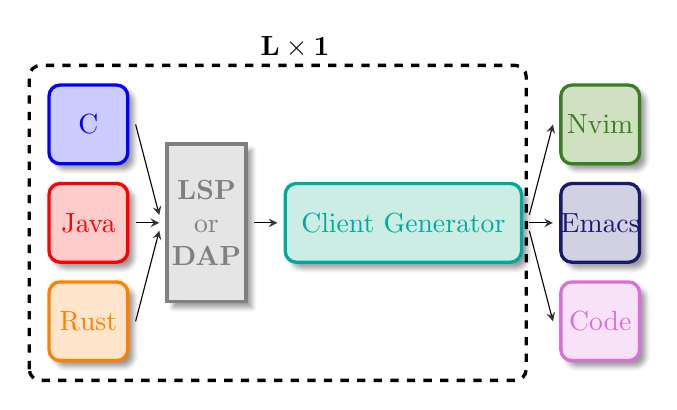
\begin{tikzpicture}

% \draw[dashed, very thick, rounded corners, anchor=north]
%         (-0.25,-0.25) rectangle (3.5,3.75)
%         node[anchor=north, align=center] at (1.75,4.25) {$\mathbf{L} \times \mathbf{E}$};
% \draw[dashed, very thick, rounded corners, anchor=north]
%         (3.75,-0.25) rectangle (8.25,3.75)
%         node[anchor=north, align=center] at (6.125,4.25) {$\mathbf{L} + \mathbf{E}$};

\draw[dashed, very thick, rounded corners, anchor=north]
        (3.75,-0.25) rectangle (10.06, 3.75)
        node[anchor=north, align=center] at (7.125,4.25) {$\mathbf{L} \times \mathbf{1}$};
%
% % Languages
% \draw[orange, very thick, rounded corners, fill=orange!20, blur shadow={shadow blur steps=5}]
%         (0,0) rectangle (1,1)
%         node[pos=.5] {Rust};
% \draw[red, very thick, rounded corners, fill=red!20, blur shadow={shadow blur steps=5}]
%         (0,1.25) rectangle (1,2.25)
%         node[pos=.5] {Java};
% \draw[blue, very thick, rounded corners, fill=blue!20, blur shadow={shadow blur steps=5}]
%         (0,2.5) rectangle (1,3.5)
%         node[pos=.5] {C};
% % Editors
% \draw[Orchid, very thick, rounded corners, fill=Orchid!20, blur shadow={shadow blur steps=5}]
%         (2.25,0) rectangle (3.25,1)
%         node[pos=.5] {Code};
% \draw[OliveGreen, very thick, rounded corners, fill=OliveGreen!20, blur shadow={shadow blur steps=5}]
%         (2.25,2.5) rectangle (3.25,3.5)
%         node[pos=.5] {Nvim};
% \draw[MidnightBlue, very thick, rounded corners, fill=MidnightBlue!20, blur shadow={shadow blur steps=5}]
%         (2.25,1.25) rectangle (3.25,2.25)
%         node[pos=.5] {Emacs};
% % Connections
% % C
% \draw[->, >=stealth] (1.1,3) -- (2.20,3); %
% \draw[->, >=stealth] (1.1,2.9) -- (2.20,1.85);
% \draw[->, >=stealth] (1.1,2.8) -- (2.20,0.7);
% % Java
% \draw[->, >=stealth] (1.1,1.85) -- (2.20,2.9);
% \draw[->, >=stealth] (1.1,1.75) -- (2.20,1.75); %
% \draw[->, >=stealth] (1.1,1.65) -- (2.20,0.6);
% % Rust
% \draw[->, >=stealth] (1.1,0.7) -- (2.20,2.8);
% \draw[->, >=stealth] (1.1,0.6) -- (2.20,1.65);
% \draw[->, >=stealth] (1.1,0.5) -- (2.20,0.5); %

% Languages
\draw[blue, very thick, rounded corners, fill=blue!20, blur shadow={shadow blur steps=5}]
(4,2.5) rectangle (5,3.5)
node[pos=.5] {C};
\draw[red, very thick, rounded corners, fill=red!20, blur shadow={shadow blur steps=5}]
        (4,1.25) rectangle (5,2.25)
        node[pos=.5] {Java};
\draw[orange, very thick, rounded corners, fill=orange!20, blur shadow={shadow blur steps=5}]
        (4,0) rectangle (5, 1)
        node[pos=.5] {Rust};
% LSP
\draw[gray, very thick, fill=gray!20, blur shadow={shadow blur steps=5}]
        (5.5, 0.75) rectangle (6.5, 2.75)
        node[text width=4cm, pos=.5, align=center] {\textbf{LSP} \linebreak or \linebreak \textbf{DAP}};

% Client Generator
\draw[Emerald, very thick, rounded corners, fill=Emerald!20, blur shadow={shadow blur steps=5}]
        (7,1.25) rectangle (10,2.25)
        node[pos=.5] {Client Generator};

% Editors
\draw[Orchid, very thick, rounded corners, fill=Orchid!20, blur shadow={shadow blur steps=5}]
        (10.5,0) rectangle (11.5,1)
        node[pos=.5] {Code};
\draw[OliveGreen, very thick, rounded corners, fill=OliveGreen!20, blur shadow={shadow blur steps=5}]
        (10.5,2.5) rectangle (11.5,3.5)
        node[pos=.5] {Nvim};
\draw[MidnightBlue, very thick, rounded corners, fill=MidnightBlue!20, blur shadow={shadow blur steps=5}]
        (10.5,1.25) rectangle (11.5,2.25)
        node[pos=.5] {Emacs};
% Connections
\draw[->, >=stealth] (5.1,3)      -- (5.4,1.85);
\draw[->, >=stealth] (5.1,1.75)   -- (5.4,1.75);
\draw[->, >=stealth] (5.1,0.5)    -- (5.4,1.65);

% \draw[->, >=stealth] (6.6, 1.85) -- (6.9, 3);
\draw[->, >=stealth] (6.6, 1.75) -- (6.9, 1.75);
% \draw[->, >=stealth] (6.6, 1.65) -- (6.9, 0.5);

\draw[->, >=stealth] (10.1, 1.85) -- (10.4, 3);
\draw[->, >=stealth] (10.1, 1.75) -- (10.4, 1.75);
\draw[->, >=stealth] (10.1, 1.65) -- (10.4, 0.5);

\end{tikzpicture}

\end{document}


